\documentclass{beamer}
 
\usepackage{amsmath}
\usepackage[utf8]{inputenc}
\usepackage{svg}
 
\setbeamerfont{title}{family=\fontfamily{bch}\selectfont}
\setbeamerfont{frametitle}{family=\fontfamily{bch}\selectfont}
\setbeamerfont{framesubtitle}{family=\fontfamily{bch}\selectfont}
\renewcommand{\sfdefault}{qhv}
\usefonttheme{professionalfonts}



\AtBeginSection[]{
  \begin{frame}
  \vfill
  \centering
  \begin{beamercolorbox}[sep=8pt,center,shadow=true,rounded=true]{title}
    \usebeamerfont{title}\insertsectionhead\par%
  \end{beamercolorbox}
  \vfill
  \end{frame}
}

\AtBeginSubsection[]{
  \begin{frame}
  \vfill
  \centering
  \begin{beamercolorbox}[sep=8pt,center,shadow=true,rounded=true]{title}
    \usebeamerfont{title}\insertsectionhead\par%
  \end{beamercolorbox}
  \vfill
  \end{frame}
}




%%% https://tex.stackexchange.com/questions/223200/how-to-completely-remove-footer-in-beamer:
 %gets rid of bottom navigation bars
\setbeamertemplate{footline}[frame number]{}

%gets rid of bottom navigation symbols
\setbeamertemplate{navigation symbols}{}

%gets rid of footer
%will override 'frame number' instruction above
%comment out to revert to previous/default definitions
\setbeamertemplate{footline}{}
%%%

% https://tex.stackexchange.com/questions/137022/how-to-insert-page-number-in-beamer-navigation-symbols
\addtobeamertemplate{navigation symbols}{}{%
    \usebeamerfont{footline}%
    \usebeamercolor[fg]{footline}%
    \hspace{1em}%
    \insertframenumber/\inserttotalframenumber
}
 
%Information to be included in the title page:
\title{Metrology \& many-body physics with ultracold Helium}
\author{}
\institute{He* BEC group, LPC}
\date{}
 
 
 
\begin{document}
 



\section*{Introduction}

% BEGIN BLACK BACKGROUND
{\setbeamercolor{background canvas}{bg = black}
\begin{frame}{}
\begin{center}
    \begin{figure}[h]
        \includegraphics[width=.7\textwidth]{figures/Intro/Sun.jpg}
    \end{figure}
    \begin{figure}[b]
        \includegraphics[width=0.4\textwidth]{figures/Intro/Spectrum.jpg}
    \end{figure}
\end{center}
    %https://thumbor.forbes.com/thumbor/960x0/https%3A%2F%2Fblogs-images.forbes.com%2Fkionasmith%2Ffiles%2F2017%2F08%2FHelium_spectrum.jpg - NASA
    % Second-most abundant element in the universe, 23 per cent of baryonic mass, produced within the first three minutes of the universe's existence; only 5.2ppm in earth's atmosphere
    % Most terrestrial helium is produced by Alpha decay, producing the most stable known nucleus
 %Helium is named for the Greek Titan of the Sun, Helios. It was first detected as an unknown yellow spectral line signature in sunlight during a solar eclipse in 1868 by Georges Rayet,[5] Captain C. T. Haig,[6] Norman R. Pogson,[7] and Lieutenant John Herschel,[8] and was subsequently confirmed by French astronomer Jules Janssen.[9] Janssen is often jointly credited with detecting the element along with Norman Lockyer. Janssen recorded the helium spectral line during the solar eclipse of 1868 while Lockyer observed it from Britain. Lockyer was the first to propose that the line was due to a new element, which he named. The formal discovery of the element was made in 1895 by two Swedish chemists, Per Teodor Cleve and Nils Abraham Langlet, who found helium emanating from the uranium ore cleveite. In 1903, large reserves of helium were found in natural gas fields in parts of the United States, which is by far the largest supplier of the gas today. - wiki
  
  % 587.49nm line, $1s2p ^3P \rightarrow 1s3d 1D \& 3D$ probably blurring of both
  
  %Mark Oliphant transmuted Lithium to Helium at the Cavendish laboratory 1n 1932-33, bombarding Lithium with protons, providing the first experimental evidence of nuclear fusion and identifying H3 and He3
  
  % He3 is fermionic, He4 is bosonic
\end{frame}


%% Replace with atom lasers, they're more relevant to early talk?
\begin{frame}{}
\begin{center}
    \begin{figure}[h]
        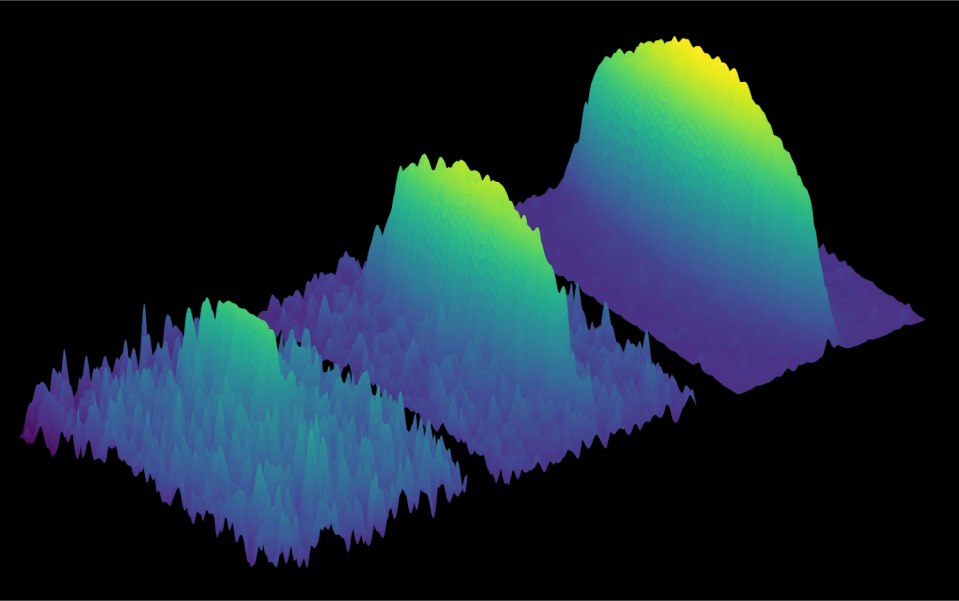
\includegraphics[width=\textwidth]{figures/Intro/BEC.png}
    \end{figure}
\end{center}
\end{frame}
}%% END BLACK BACKGROUND


\begin{frame}{The cold atom zoo\footnote[frame]{everycoldatom.com}}
     \begin{center}
    \includegraphics[width=\textwidth]{figures/Intro/all_cold_elements.png}
     \end{center}

\end{frame}


\begin{frame}{The world of ultracold atoms\footnote[frame]{everycoldatom.com}}
    \begin{center}
        \includegraphics[width=\textwidth]{figures/Intro/every_cold_atom.png}
    \end{center}
     
\end{frame}


\frame{\titlepage}

\begin{frame}{What good are BECs?}
    They're excellent testbeds for fundamental physics.\vspace{1in}
    
    They exhibit controllable macroscopic coherent phenomena.\vspace{1in}
    
    They're rich resources for engineering `large' quantum states.
\end{frame}

% \begin{frame}{Contents}
%     \tableofcontents
% \end{frame}

{
\usebackgroundtemplate{\includegraphics[width=\paperwidth]{figures/Intro/apparatus.png}}%
\begin{frame}{Our apparatus}
    \begin{figure}[b]
        \centering
        % \includegraphics[width=\paperwidth]{figures/Intro/apparatus.png}
    \end{figure}
\end{frame}
}

% %% Laser cooling section
% \begin{frame}{Cooling to BEC: Doppler cooling}
%     \begin{figure}
%         \centering
%         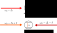
\includegraphics{figures/Intro/Cooling/doppler_cooling.png}
%         % \caption{Caption}
%         \label{fig:my_label}
%     \end{figure}
% \end{frame}
% \begin{frame}{Cooling to BEC: Optical molasses}
%     \begin{figure}
%         \centering
%         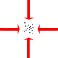
\includegraphics{figures/Intro/Cooling/optical_molasses.png}
%         % \caption{Caption}
%         \label{fig:my_label}
%     \end{figure}
% \end{frame}
% \begin{frame}{Cooling to BEC: Magneto-Optical trapping}
%     \begin{figure}
%         \centering
%         \includegraphics{figures/Intro/Cooling/MOT.png}
%         % \caption{Caption}
%         \label{fig:my_label}
%     \end{figure}
% \end{frame}
% \begin{frame}{Cooling to BEC: Magnetic trapping \& Evaporation}
%     \begin{figure}
%         \centering
%         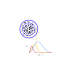
\includegraphics{figures/Intro/Cooling/evap_1.png}
%         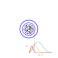
\includegraphics{figures/Intro/Cooling/evap_2.png}
%         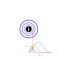
\includegraphics{figures/Intro/Cooling/evap_3.png}
%         % \caption{Caption}
%         \label{fig:my_label}
%     \end{figure}
% \end{frame}


%% end laser cooling

\begin{frame}{Helium}
     \begin{center}
    \includegraphics[width=\textwidth]{figures/spectroscopy_level_diagram.png}
     \end{center}
\end{frame}

\begin{frame}{Single-atom detection}
\begin{figure}
    \centering
    \includegraphics[width=0.5\textwidth]{figures/Intro/detector.png}
    \includegraphics[width=0.5\textwidth]{figures/Intro/dld_schematic.png}
    % \caption{Caption}
    \label{fig:my_label}
\end{figure}    
\end{frame}

\section{Metrology I: Transition spectroscopy}


% \begin{frame}{Helium}
%      \begin{center}
%     \includegraphics[width=\textwidth]{figures/spectroscopy_level_diagram.png}
%      \end{center}
% \end{frame}

% \begin{frame}{Motivation}
%     \begin{itemize}
%         \item Precision spectroscopy and accurate theory enable atomic tests of QED
%         \item High-lying states have less theoretical uncertainty, but aren't currently accessible from the ground state
%         \item There are known disagreements between predicted and observed intervals involving the $n=2\rightarrow 5D$ transitions
%         \item Presently, theory and experiment disagree over the singlet-triplet interval in Helium.
%     \end{itemize}
% \end{frame}

\begin{frame}{On needles in haystacks}
    \begin{center}
        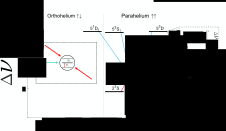
\includegraphics[width=\textwidth]{figures/Spectra/spectroscopy_targets.png}    
    \end{center}
\end{frame}

\begin{frame}{Experimental schematic}
    \begin{center}
        \includegraphics[width=0.8\textwidth]{figures/expt_schematic_simplified.png}    
    \end{center}
\end{frame}

\begin{frame}{Measurement sequence}
    \begin{figure}
        \centering
        \includegraphics[width=\textwidth]{figures/Spectra/spectroscopy_sequence.png}
        % \caption{Caption}
        % Label curves with words
        % Add cartoon and level diagram to explain: signal, gain, response measurement
        \label{fig:my_label}
    \end{figure}
\end{frame}

% Label plots with words
\begin{frame}{Transition spectra}
    \begin{center}
        \includegraphics[width=0.8\textwidth]{figures/Spectra/5^1D_2_plot_combo.png}    
    \end{center}
\end{frame}

\begin{frame}{Transition spectra}
    \begin{center}
        \includegraphics[width=0.9\textwidth]{figures/Spectra/lines_combined.png}    
    \end{center}
\end{frame}

\begin{frame}{Spectroscopic results}
% Add wavelengths
    \begin{center}
        \begin{tabular}{|c||c|c|c|}
        \hline
            $|e\rangle$ &  $\nu_{obs}$ (MHz)    &$\nu_{obs}-\nu_{theory}$ (MHz) \\
            \hline\hline
            $5^3\mathrm{S}_1$ & 727303247.812(0.143)    & 3.212\\
            $5^3\mathrm{D}_1$ & 744396515.588(0.224)     & 4.448\\
            $5^3\mathrm{D}_2$ & 744396235.844(0.282)   & 8.264\\
            $5^3\mathrm{D}_3$ & 744396204.115(0.341)   &-4.245\\
            $5^1\mathrm{D}_2$ & 744430345.471(0.047)     &	2.121\\
            \hline
        \end{tabular}
        % Old measurements by William Martin, New Wavelengths for Some Helium (He i) Lines
        % Journal of the Optical Society of America Vol. 50, Issue 2, pp. 174-176 (1960)
\end{center}
\end{frame}
\begin{frame}{Systematics \& past results}
    \begin{center}
        \begin{tabular}{|c||c|c|c|}
        \hline
            $|e\rangle$ &  $\nu_{obs}$ (MHz)     & $ \nu_{obs} - \nu_{old}$\footnote[frame]{Martin, New Wavelengths for Some Helium (He i) Lines, Journal of the Optical Society of America Vol. 50, Issue 2, pp. 174-176 (1960)} (MHz) \\
        \hline\hline
            $5^3\mathrm{S}_1$    & 727303247(4)        & 13713(201)\\
            $5^3\mathrm{D}_1$    & 744396515(20)        & 13575(168)\\
            $5^3\mathrm{D}_2$    & 744396235(20)        & 13855(168)\\
            $5^3\mathrm{D}_3$    & 744396204(20)        & 13886(168)\\
            $5^1\mathrm{D}_2$    & 744430345(20)        & N/A\\
            \hline
        \end{tabular}
    \end{center}
    
% Old measurements by William Martin, New Wavelengths for Some Helium (He i) Lines
% Journal of the Optical Society of America Vol. 50, Issue 2, pp. 174-176 (1960)
\end{frame}

\section{Metrology II: Tuneout}
% \begin{frame}{Motivation}
%     \begin{itemize}
%         \item Single-point absolute reference
%         \item No need for absolute intensity calibration
%         \item Sum over all orbitals means very stringent test for QED
%         \item Present theory is sufficiently advanced to include high-order QED corrections
%     \end{itemize}
% \end{frame}

\begin{frame}{Tuneout wavelengths\footnote[frame]{Henson et al, PRL 115 (2015)}}
    \begin{center}
        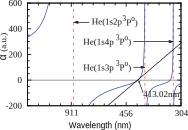
\includegraphics[width=0.8\textwidth]{figures/TO/plz.png}    
    \end{center}
    $$
    U_{light} = -\frac{\alpha(\nu)}{2}\langle\mathcal{E}^2\rangle
    $$
\end{frame}

% \begin{frame}{Polarizability}
%     \begin{itemize}
%         \item Dipole response to electric field gives rise to optical potential
%         \item Trap combination theory
%         \item Optical frequency shift measurement
%         \item Dependence on polarization
%     \end{itemize}
% \end{frame}

% \begin{frame}{Experimental schematic}
%     \begin{center}
%         \includegraphics[width=0.8\textwidth]{figures/expt_schematic_simplified.png}    
%     \end{center}
% \end{frame}

\begin{frame}{Hybrid trap response function}
    \begin{center}
        \includegraphics[width=\textwidth]{figures/TO/trap_response.png}    
    \end{center}
    

    % $$
    \begin{align}
        F &= -\nabla(U_{L} + U_{B})\\
            & =\sqrt{m  \partial_{x}\left(\alpha(\nu)|\mathcal{E}|+\mu |B|\right)} x\\
    \implies \omega &= \sqrt{\omega_{B}^2 + \omega_{E}^2}
    \end{align}
    % $$
\end{frame}


% \begin{frame}{Measurement sequence}
%     \begin{figure}
%         \centering
%         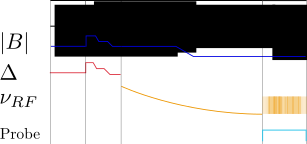
\includegraphics[width=\textwidth]{figures/TO/TO_sequence.png}
%         % \caption{Caption}
%         \label{fig:my_label}
%     \end{figure}
% \end{frame}


% \begin{frame}{Determining the Tuneout wavelength}
%     \begin{center}
%         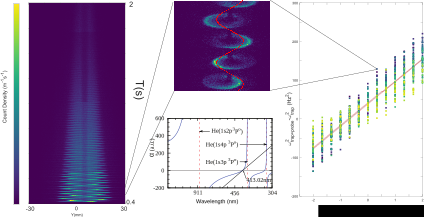
\includegraphics[width=\textwidth]{figures/TO/t_freq_fit.png}    
%     \end{center}
% \end{frame}

% \begin{frame}{Determining the Tuneout wavelength}

% % Li Yan's equation
% The dynamic polarizability depends on the frequency $(\omega)$ and polarization of light:
% $$
%     \alpha(\omega) = \alpha^s(\omega) + C \alpha^v(\omega) \frac{M}{2J} + D \alpha^T(\omega) \frac{3M^2-J(J+1)}{2J(2J-1)}
% $$

% Where $C = -V \cos(\theta_k)$ and $D = \frac{3}\sin^2(\theta_k) (1 + Q)$

% Which permits an expression for the Tuneout:
% $$
%     \omega_{to} = \omega_{s,0} + \frac{1}{2} \omega^T + \frac{1}{2} \mathcal{V} \cos \left( \theta_k \right) \omega^v - \frac{3}{2} \mathcal{P} \sin^2(\theta_k) \omega^T.
% $$

% % Poincare sphere graphic
 
% \end{frame}


% \begin{frame}{Determining the Tuneout wavelength}
%     \begin{center}
%         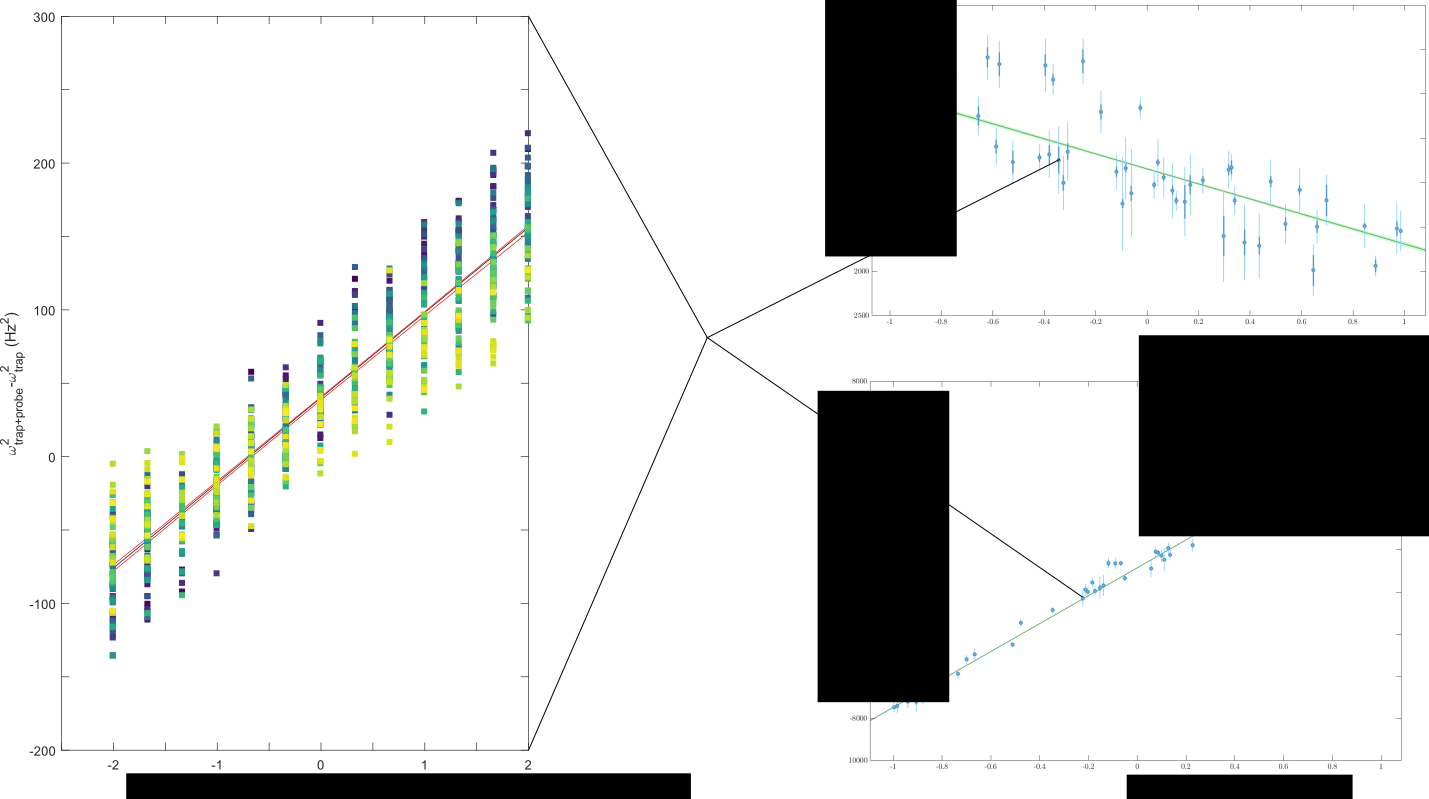
\includegraphics[width=\textwidth]{figures/TO/polz_dep_compute.png}    
%     \end{center}
% \end{frame}

\begin{frame}{Results...}

\end{frame}

\begin{frame}{Results... coming soon!}

\end{frame}

\section{Many-Body physics I: Quantum depletion}
% Interactions matter. Cold atoms allow for control over their importance & investigation of emergent many-body physics, from weakly to strongly correlated systems.
% \subsection{Quantum depletion}

\begin{frame}{What is depletion?}

Thermodynamics forbids a pure condensate. Instead, they coexist with a `depleted' population:
\begin{center}
        $|\Psi\rangle = \psi_0  + \hat{\delta\psi},$ where $\psi_0 = \sqrt{N_0}e^{i\theta}$    
\end{center}
The Gross-Pitaevskii equation describes the dynamics of the condensed fraction:
        $$
            i\hbar\frac{\partial\psi_0}{\partial t} = \left(-\frac{\hbar^2}{2m}\nabla^2+V+g|\psi_0|^2\right)\psi_0
        $$
Quantum depletion is the `quantum correction' to $\psi_0$, whose amplitude scales with the \textit{gas parameter} $\sqrt{n a_{s}^3}$

\end{frame}

\begin{frame}{Quantum depletion in the wild}
    \begin{itemize}
        \item First observation in an optical lattice\footnote[frame]{Xu et al, PRL 96 (2006)}
        \item More recently observed in a homogenous trap\footnote[frame]{Lopes et al, PRL 119 (2017)}
    \end{itemize}

    \begin{center}
        % \includegraphics[scale=0.6]{figures/QD/xu_profile.png}
        \includegraphics[scale=0.6]{figures/QD/xu_results.png}    
        \includegraphics[scale=0.6]{figures/QD/Lopez_results.png}  
    \end{center}
\end{frame}

% \begin{frame}{Quantum depletion in the wild}
%     \begin{itemize}
%         \item Recently observed in homogeneous trap\footnote[frame]{Reference}
%         \item Feshbach resonance to control scattering length
%         \item Bragg diffraction to measure low-momentum population
%     \end{itemize}
%     \begin{center}
%         \includegraphics[scale=0.6]{figures/QD/lopes_diagram.png}
%         \includegraphics[scale=0.6]{figures/QD/lopes_profile.png}    
%     \end{center}
% \end{frame}

% \begin{frame}{Quantum depletion in the wild}
%     \begin{itemize}
%         \item Recently observed in homogeneous trap\footnote[frame]{Reference}
%         \item Feshbach resonance to control scattering length
%         \item Bragg diffraction to measure low-momentum population
%     \end{itemize}
%     \begin{center}
%         \includegraphics[scale=0.6]{figures/QD/Lopez_results.png}    
%     \end{center}
% \end{frame}

% \begin{frame}{Quantum depletion in the wild}
%     \begin{itemize}
%         \item Far-field anomaly observed in Palaiseau lab\footnote[frame]{Reference}
%         \item MCP-DLD resolves six orders of magnitude in density
%         \item Fit profile to recover depletion scale factor $n(k)\propto Ck^{-4}$
%     \end{itemize}
%     \begin{center}
%         \includegraphics[scale=0.6]{figures/QD/chang_diagram.png}  
%         \includegraphics[scale=0.6]{figures/QD/chang_profile.png}
%     \end{center}
% \end{frame}

% \begin{frame}{Quantum depletion in in far-field}
%     \begin{itemize}
%         \item Far-field anomaly observed in Palaiseau lab\footnote[frame]{Reference}
%         \item MCP-DLD resolves six orders of magnitude in density
%         \item Fit profile to recover depletion scale factor $n(k)\propto Ck^{-4}$
%     \end{itemize}
%     \begin{center}
        
%         \includegraphics[scale=0.6]{figures/QD/chang_profile.png}
%     \end{center}
% \end{frame}

% \begin{frame}{Quantum depletion in far-field}
%     \begin{itemize}
%         \item Far-field anomaly observed in Palaiseau lab\footnote[frame]{Reference}
%         \item MCP-DLD resolves six orders of magnitude in density
%         \item Fit profile to recover depletion scale factor $n(k)\propto Ck^{-4}$
%     \end{itemize}
%     \begin{center}
%         \includegraphics[scale=0.6]{figures/QD/Lopez_results.png}
%         \includegraphics[scale=0.6]{figures/QD/chang_results.png}    
%     \end{center}
% \end{frame}

\begin{frame}{Quantum depletion in far-field}
    \begin{itemize}
        \item Far-field anomaly observed in Palaiseau lab\footnote[frame]{Chang et al, PRL 117 (2016)}
        \item MCP-DLD resolves six orders of magnitude in density
        \item Fit profile to recover depletion scale factor $n(k)\propto k^{-4}$
    \end{itemize}
    \begin{center}
        \includegraphics[scale=0.6]{figures/QD/chang_profile.png} 
        \includegraphics[scale=0.6]{figures/QD/chang_results.png}    
    \end{center}
\end{frame}

% \begin{frame}{Measurement sequence}
%     \begin{center}
%          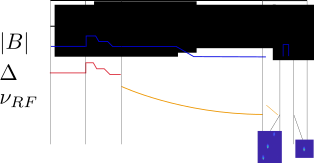
\includegraphics[width=\textwidth]{figures/QD/QD_sequence.png}  
%     \end{center}
% \end{frame}
  

\begin{frame}{Results (preliminary)}
    \begin{figure}
        \centering
        % \includegraphics[width=0.3\textwidth]{figures/QD/chang_diagram.png}  
        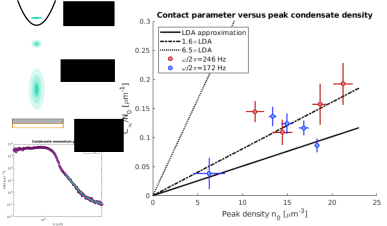
\includegraphics[width=\textwidth]{figures/QD/our_reproduction.png}  
        % \caption{Caption}
        \label{fig:my_label}
    \end{figure}
    \begin{center}
    $n_0 = \frac{m  \bar{\omega}}{8\pi\hbar a_0 }\left(\frac{15 N a_0}{a_{ho}}\right)^\frac{2}{5}$ --- $C_\infty =\frac{64\pi^2}{7}a_{0}^2N_0n_0$    
    \end{center}
\end{frame}

% \begin{frame}{What next?}
% Past experiments suggest in-trap description is quite good

% So, disagreement probably lies in early expansion. 

% We plan to investigate this regime with Bragg spectroscopy.
% \end{frame}

% \subsection{Towards an optical lattice}
\section{Many-Body physics II: Towards an optical lattice}

\begin{frame}{Motivation: Quantum simulation}
    \begin{itemize}
        \item Large-scale engineering requires accurate and efficient simulation.
        \item In general, simulating large quantum systems is intractable.
        \item Digital quantum computers would help, but are too small and noisy.
        \item Quantum simulators directly realize the Hamiltonian of a system of interest.
    \end{itemize}
\end{frame}

\begin{frame}{Optical lattices\footnote[frame]{Rispoli et al, arxiv.org/abs/1812.06959, Aidelsburger et al, Nat Phys 11 (2015)}}
    \begin{figure}
        \centering
        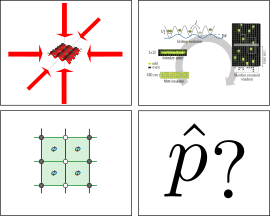
\includegraphics[width=0.8\textwidth]{figures/Lattice/lattice_tech.png}
        % \caption{Caption}
        \label{fig:my_label}
    \end{figure}
\end{frame}



\begin{frame}{The Bose-Hubbard model}
    \begin{figure}
        \centering
        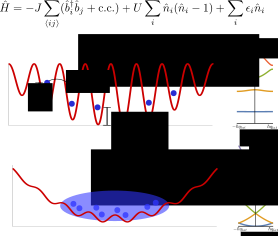
\includegraphics[width=0.8\textwidth]{figures/Lattice/potential_bands.png}
        % \caption{Caption}
        \label{fig:my_label}
    \end{figure}
\end{frame}

\begin{frame}{Building in progress...}
    \begin{figure}
        \centering
        \includegraphics[width=0.8\textwidth]{figures/Lattice/build_progress.png}
        % \caption{Caption}
        \label{fig:my_label}
    \end{figure}
\end{frame}


\begin{frame}{Coming soon...}
    % \begin{itemize}

What happens during the trap switch-off?\vspace{1in}

Can we find the forbidden $2^3\textrm{S}_1\rightarrow 3^3\textrm{S}_1$ transition?\vspace{1in}
        
Did we find a crack in the crown jewel of physics?
        

    % \end{itemize}    
\end{frame}


\begin{frame}{With thanks to...}
    \begin{itemize}
        \item \textbf{Fellow students:} Bryce Henson, David Shin, Abbas Hussein, Kieran Thomas, Sam Meng
        \item \textbf{Real doctors:} Andrew Truscott, Sean Hodgman, Ken Baldwin
        \item \textbf{Technical wizards:} Ross Tranter, Colin Dedman
        \item \textbf{Theory support:} Piotr Deuar, Gordon Drake, Li-Yan Tan
        \item And you!
    \end{itemize}
\end{frame}

 
 
 
\end{document}
